% Problem explanation
In this paper, an elastoplastic von Mises material without hardening is investigated to create a path-dependent problem. A fixed-sized square is utilized as a domain and holes of varying sizes and orientations are placed inside the domain to create different tasks. The tasks originating from different domains can be seen in Figure \ref{fig:tasks}. For all the tasks bottom part of the domain is fixed and the top part is displaced in $\dispx$ and $\dispy$ to introduce deformation to the domain (see Figure \ref{fig:problem}). After, the displacement the average Cauchy strain ($\avgstrain$) and Cauchy stress ($\avgstress$) measures are obtained for the deformation path. Then the learning problem for the $i$-th task can be defined as,
\begin{equation}
  \avgstress = f_i(\avgstrain),
\end{equation}
where a machine learning model can be utilized the find the relationship $f_i:=\avgstrain \to \avgstress$. 

% Continual Learning Problem

% Data generation
In the described problem 1000 paths for 100 displacement values are sampled for the top boundary of the domain sampled from a Gaussian Process posterior that is conditioned on 20 displacement values sampled from a uniform distribution for each path. The resulting displacement paths are utilized to obtain average stress and strains. For each presented task the same deformation paths are utilized to calculate the domain-specific average stress and strain values. The data is generated using FEniCS \cite{logg2012a}. 

% Tasks 

%Difference between tasks (I think we should present the Figures that Aleksandr showed on the difference between the tasks here.




\begin{figure}
  \centering
  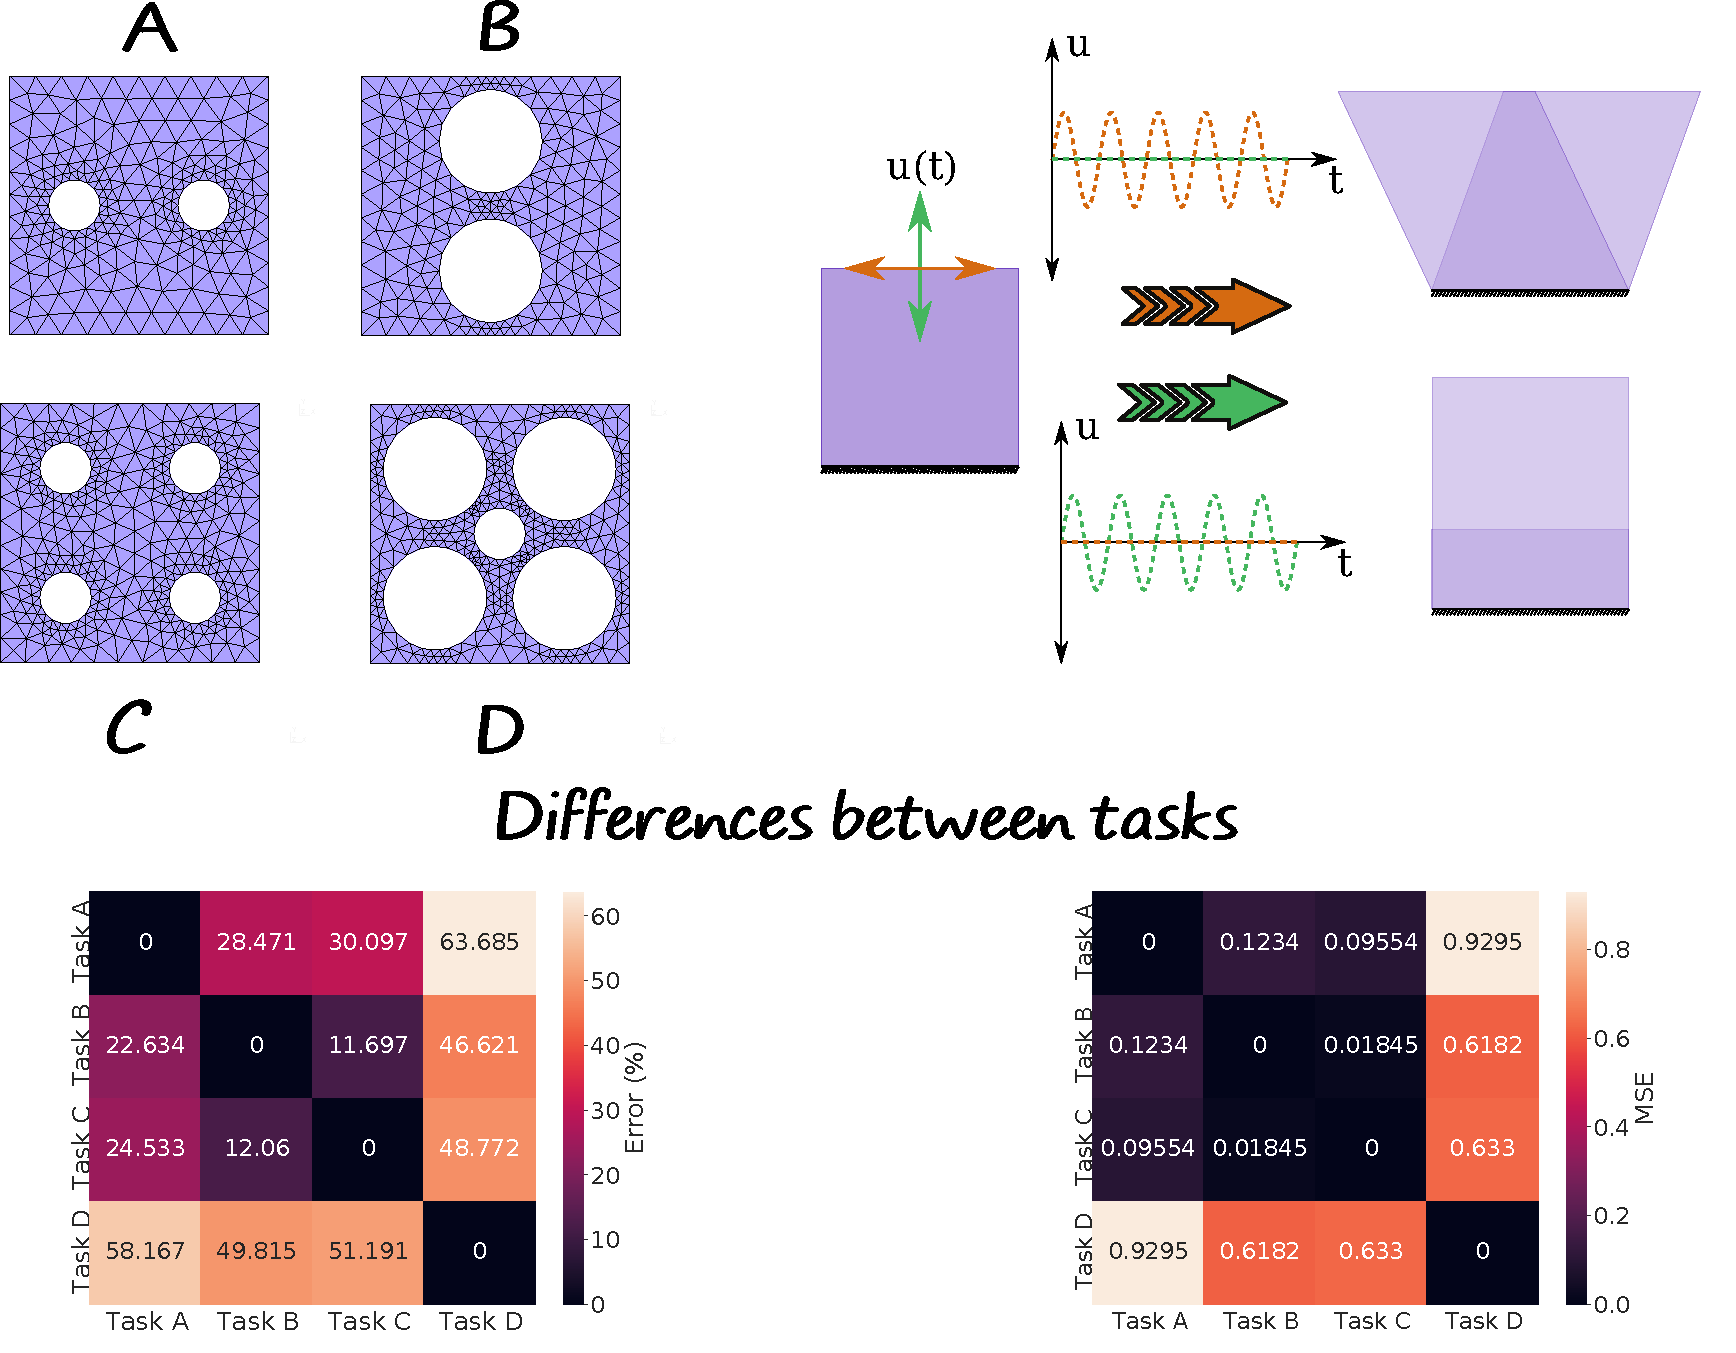
\includegraphics[scale=0.4]{Figures_\version/problem.pdf}
  \caption{A square domain with fixed on the bottom and displaced on the top. Displacement is done in a pseudo-time.}
  \label{fig:problem}
\end{figure}
\begin{figure}
  \centering
  \begin{subfigure}[b]{0.22\textwidth}
    \centering
    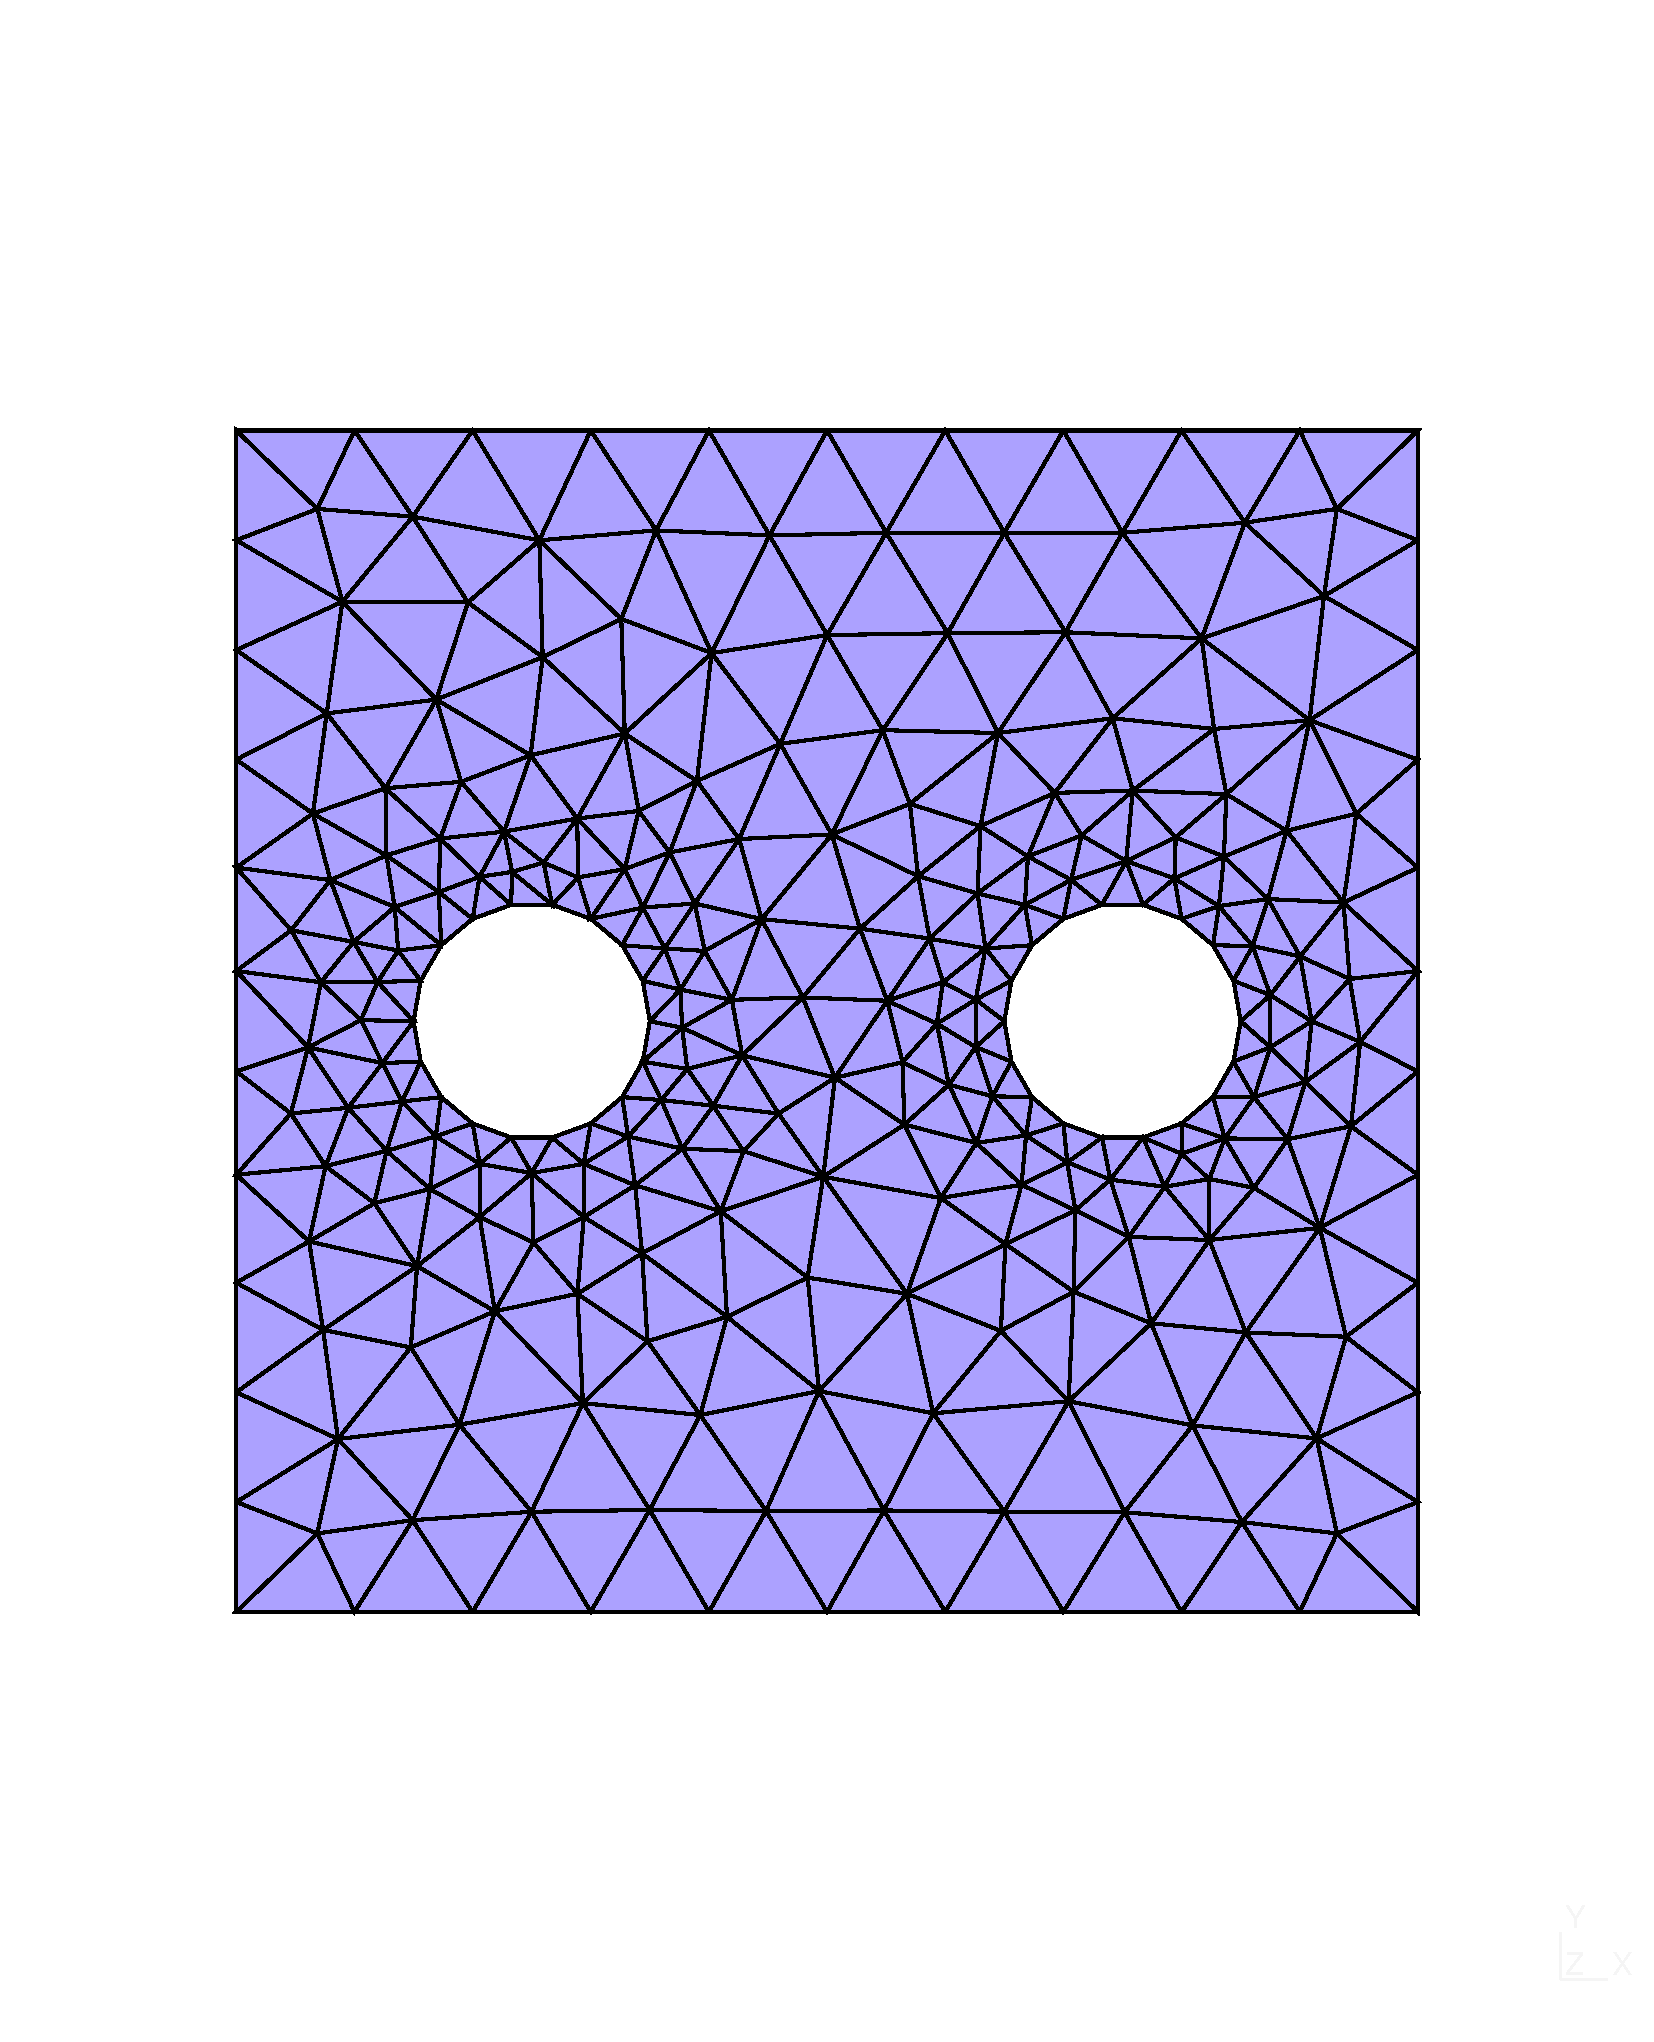
\includegraphics[width=\textwidth]{Figures_\version/tasks/2_on_x.pdf}
    \caption{Task 1}
    \label{fig:task1}
  \end{subfigure}
  \hfill
  \begin{subfigure}[b]{0.22\textwidth}
    \centering
    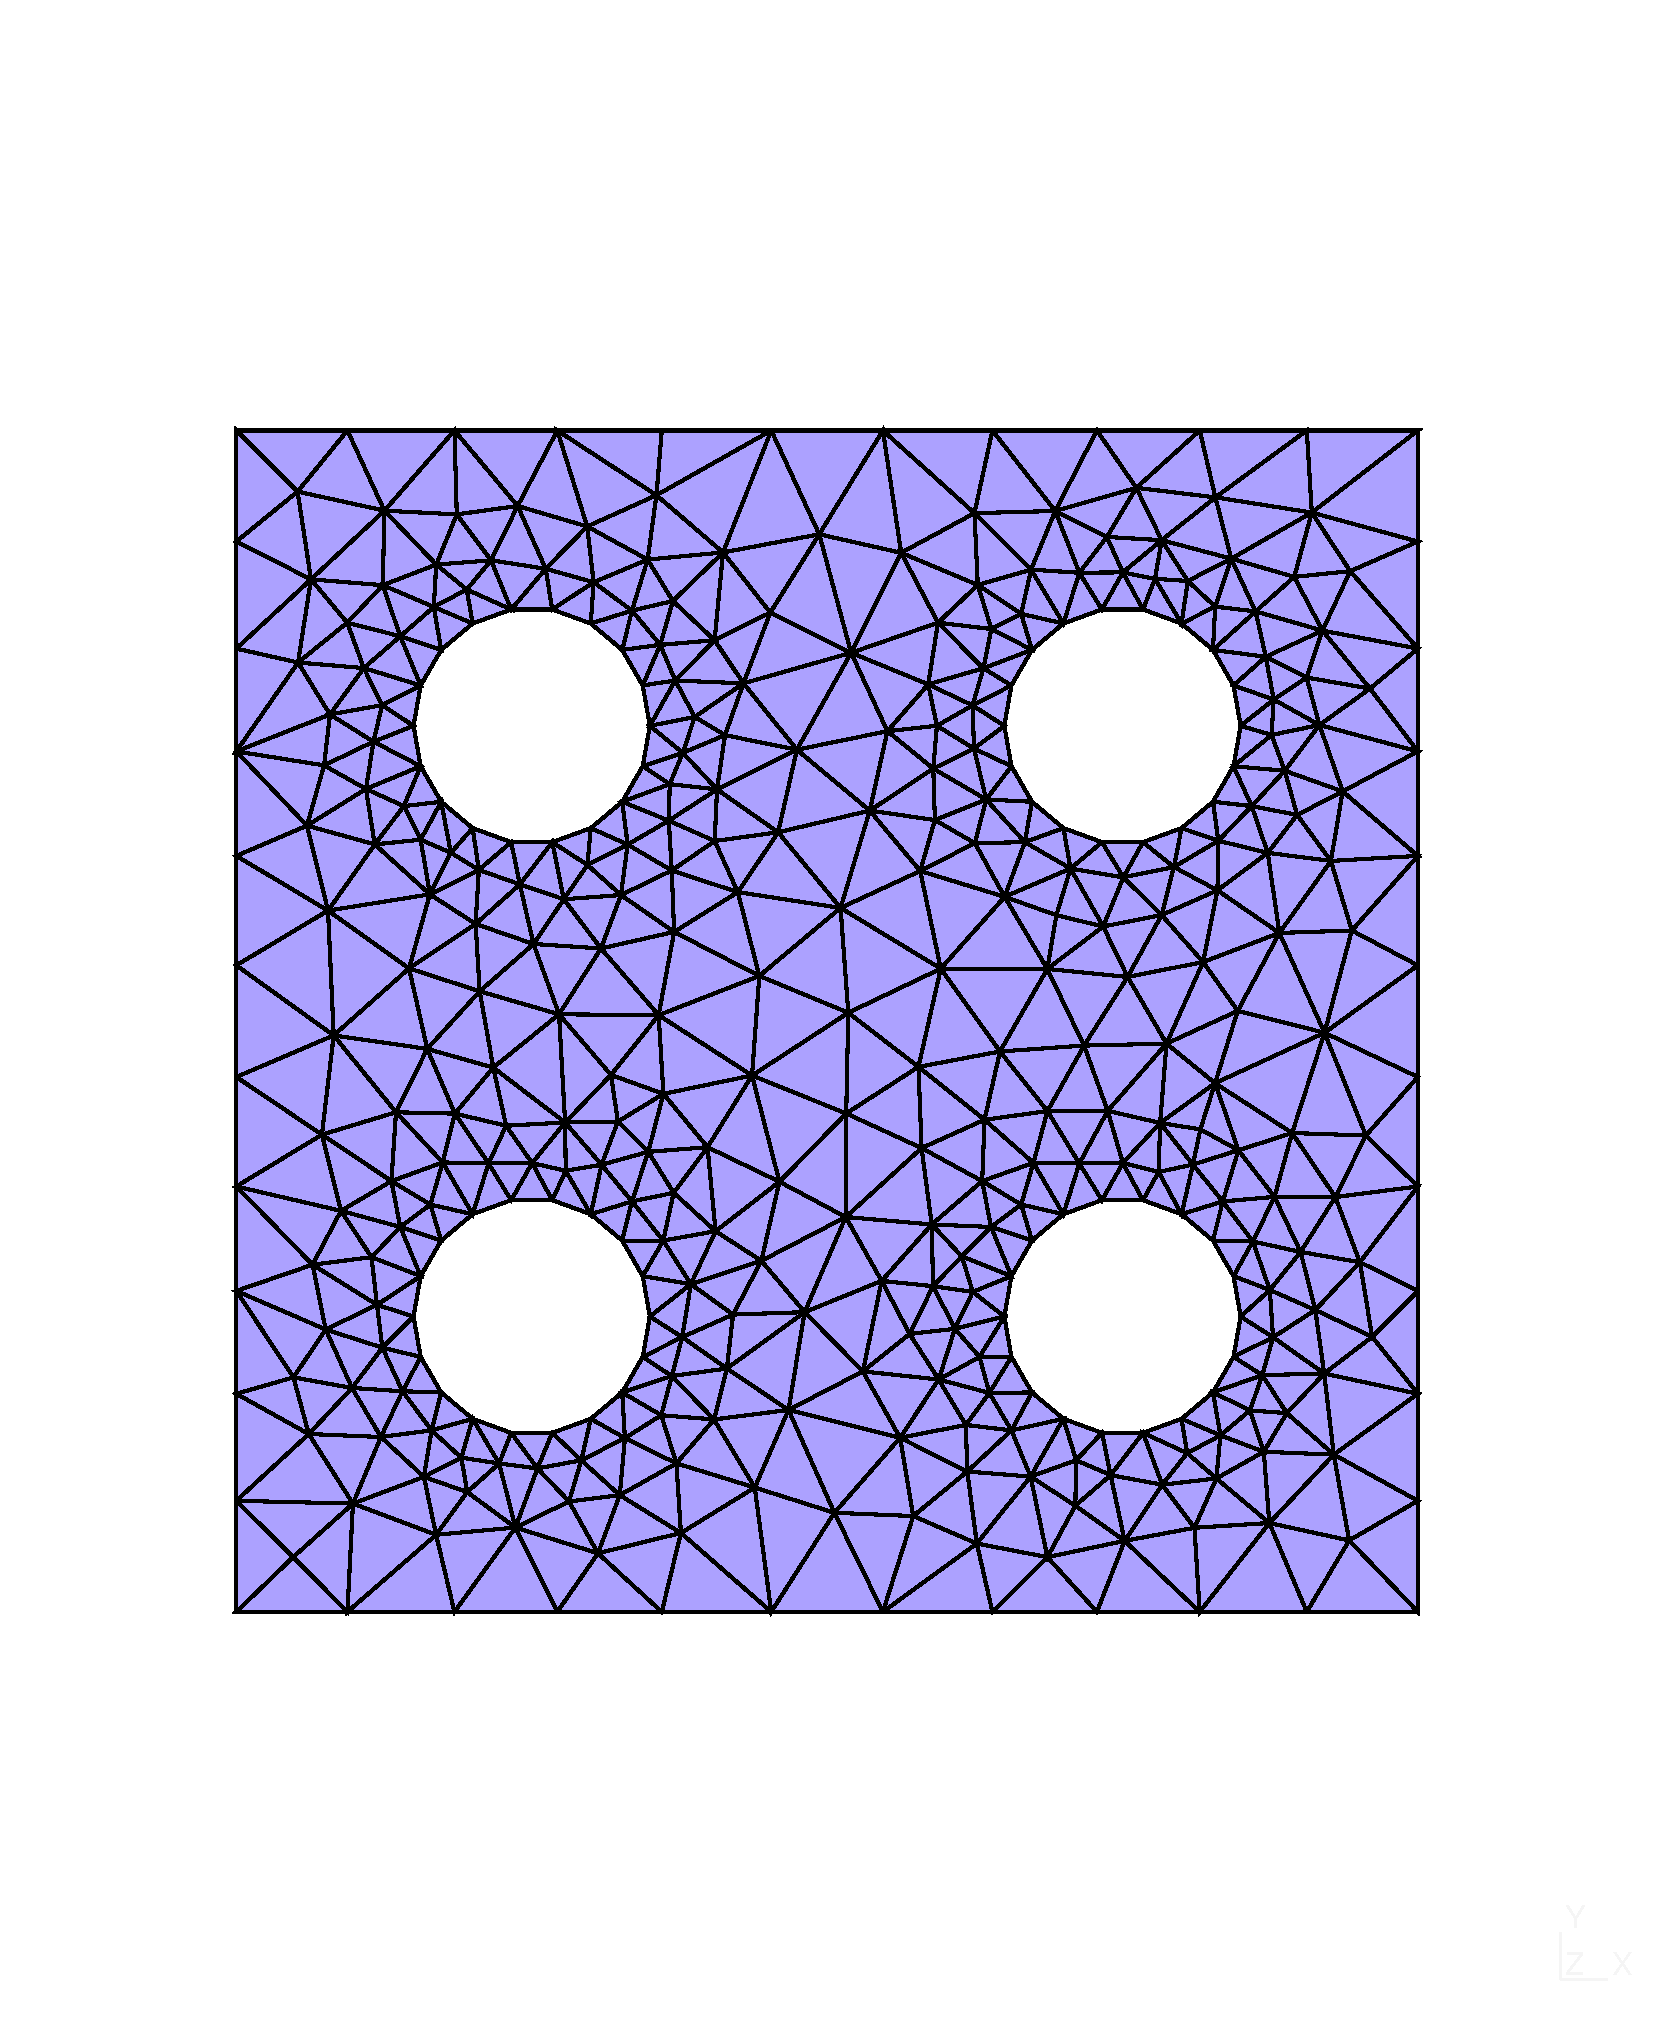
\includegraphics[width=\textwidth]{Figures_\version/tasks/4_diagonal.pdf}
    \caption{Task 2}
    \label{fig:task2}
  \end{subfigure}
  \hfill
  \begin{subfigure}[b]{0.22\textwidth}
    \centering
    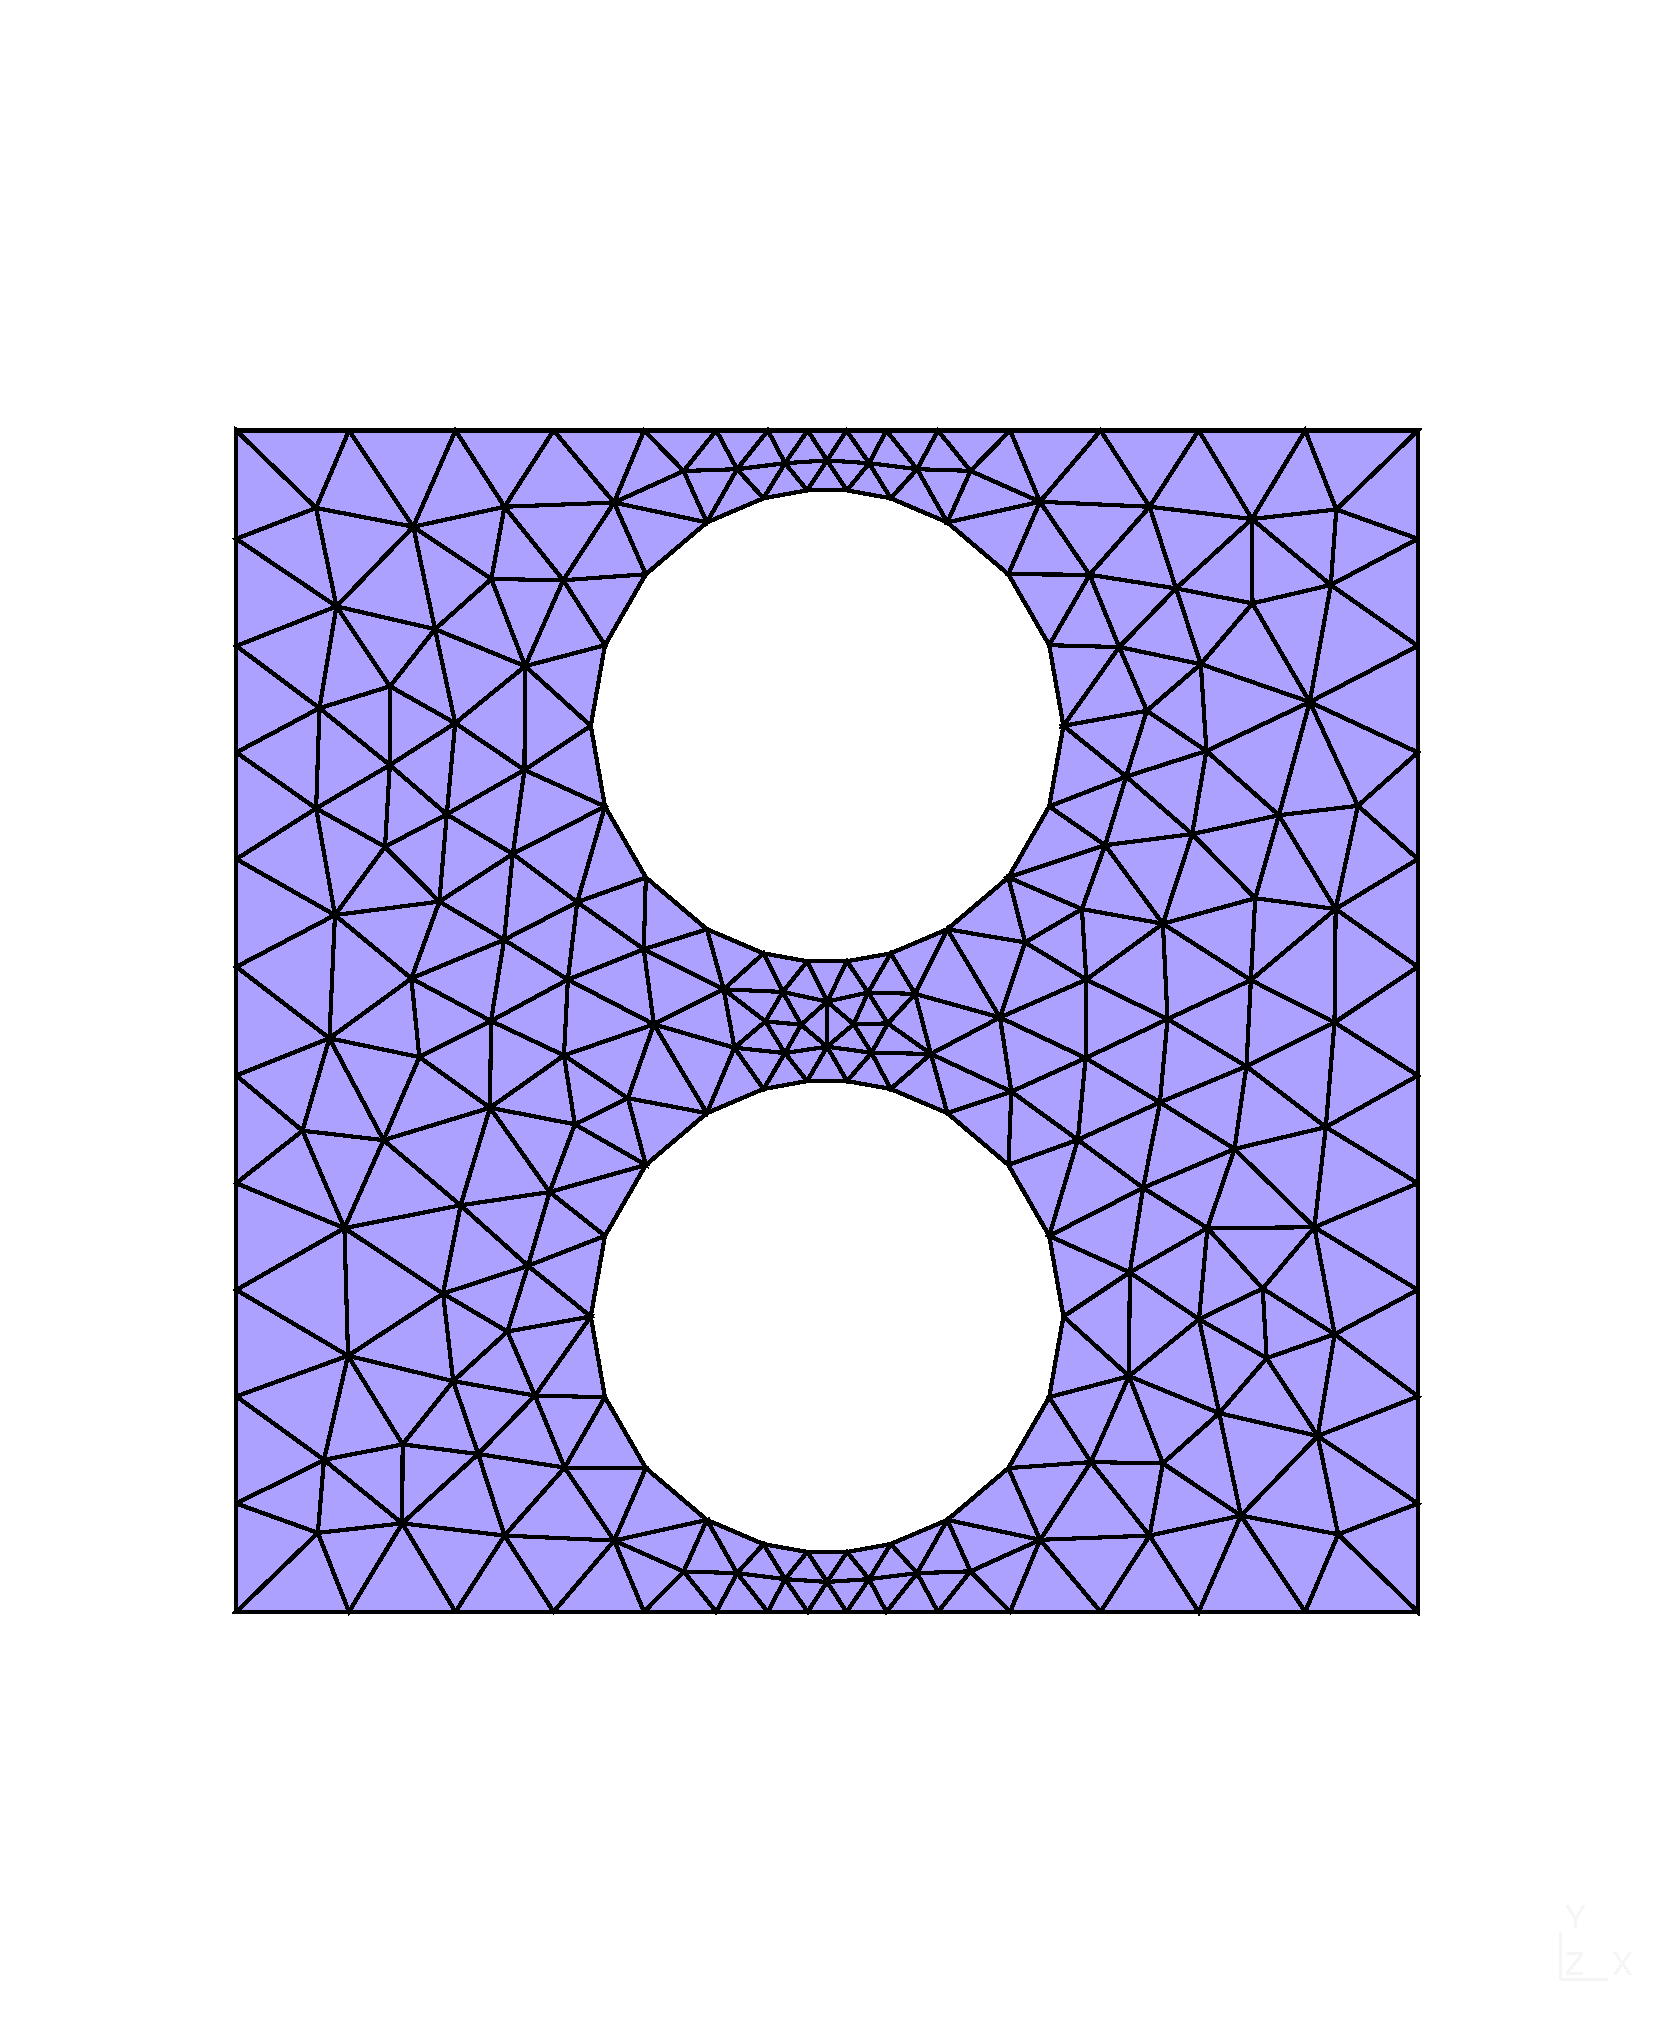
\includegraphics[width=\textwidth]{Figures_\version/tasks/2_on_y.pdf}
    \caption{Task 3}
    \label{fig:task3}
  \end{subfigure}
  \hfill
  \begin{subfigure}[b]{0.22\textwidth}
    \centering
    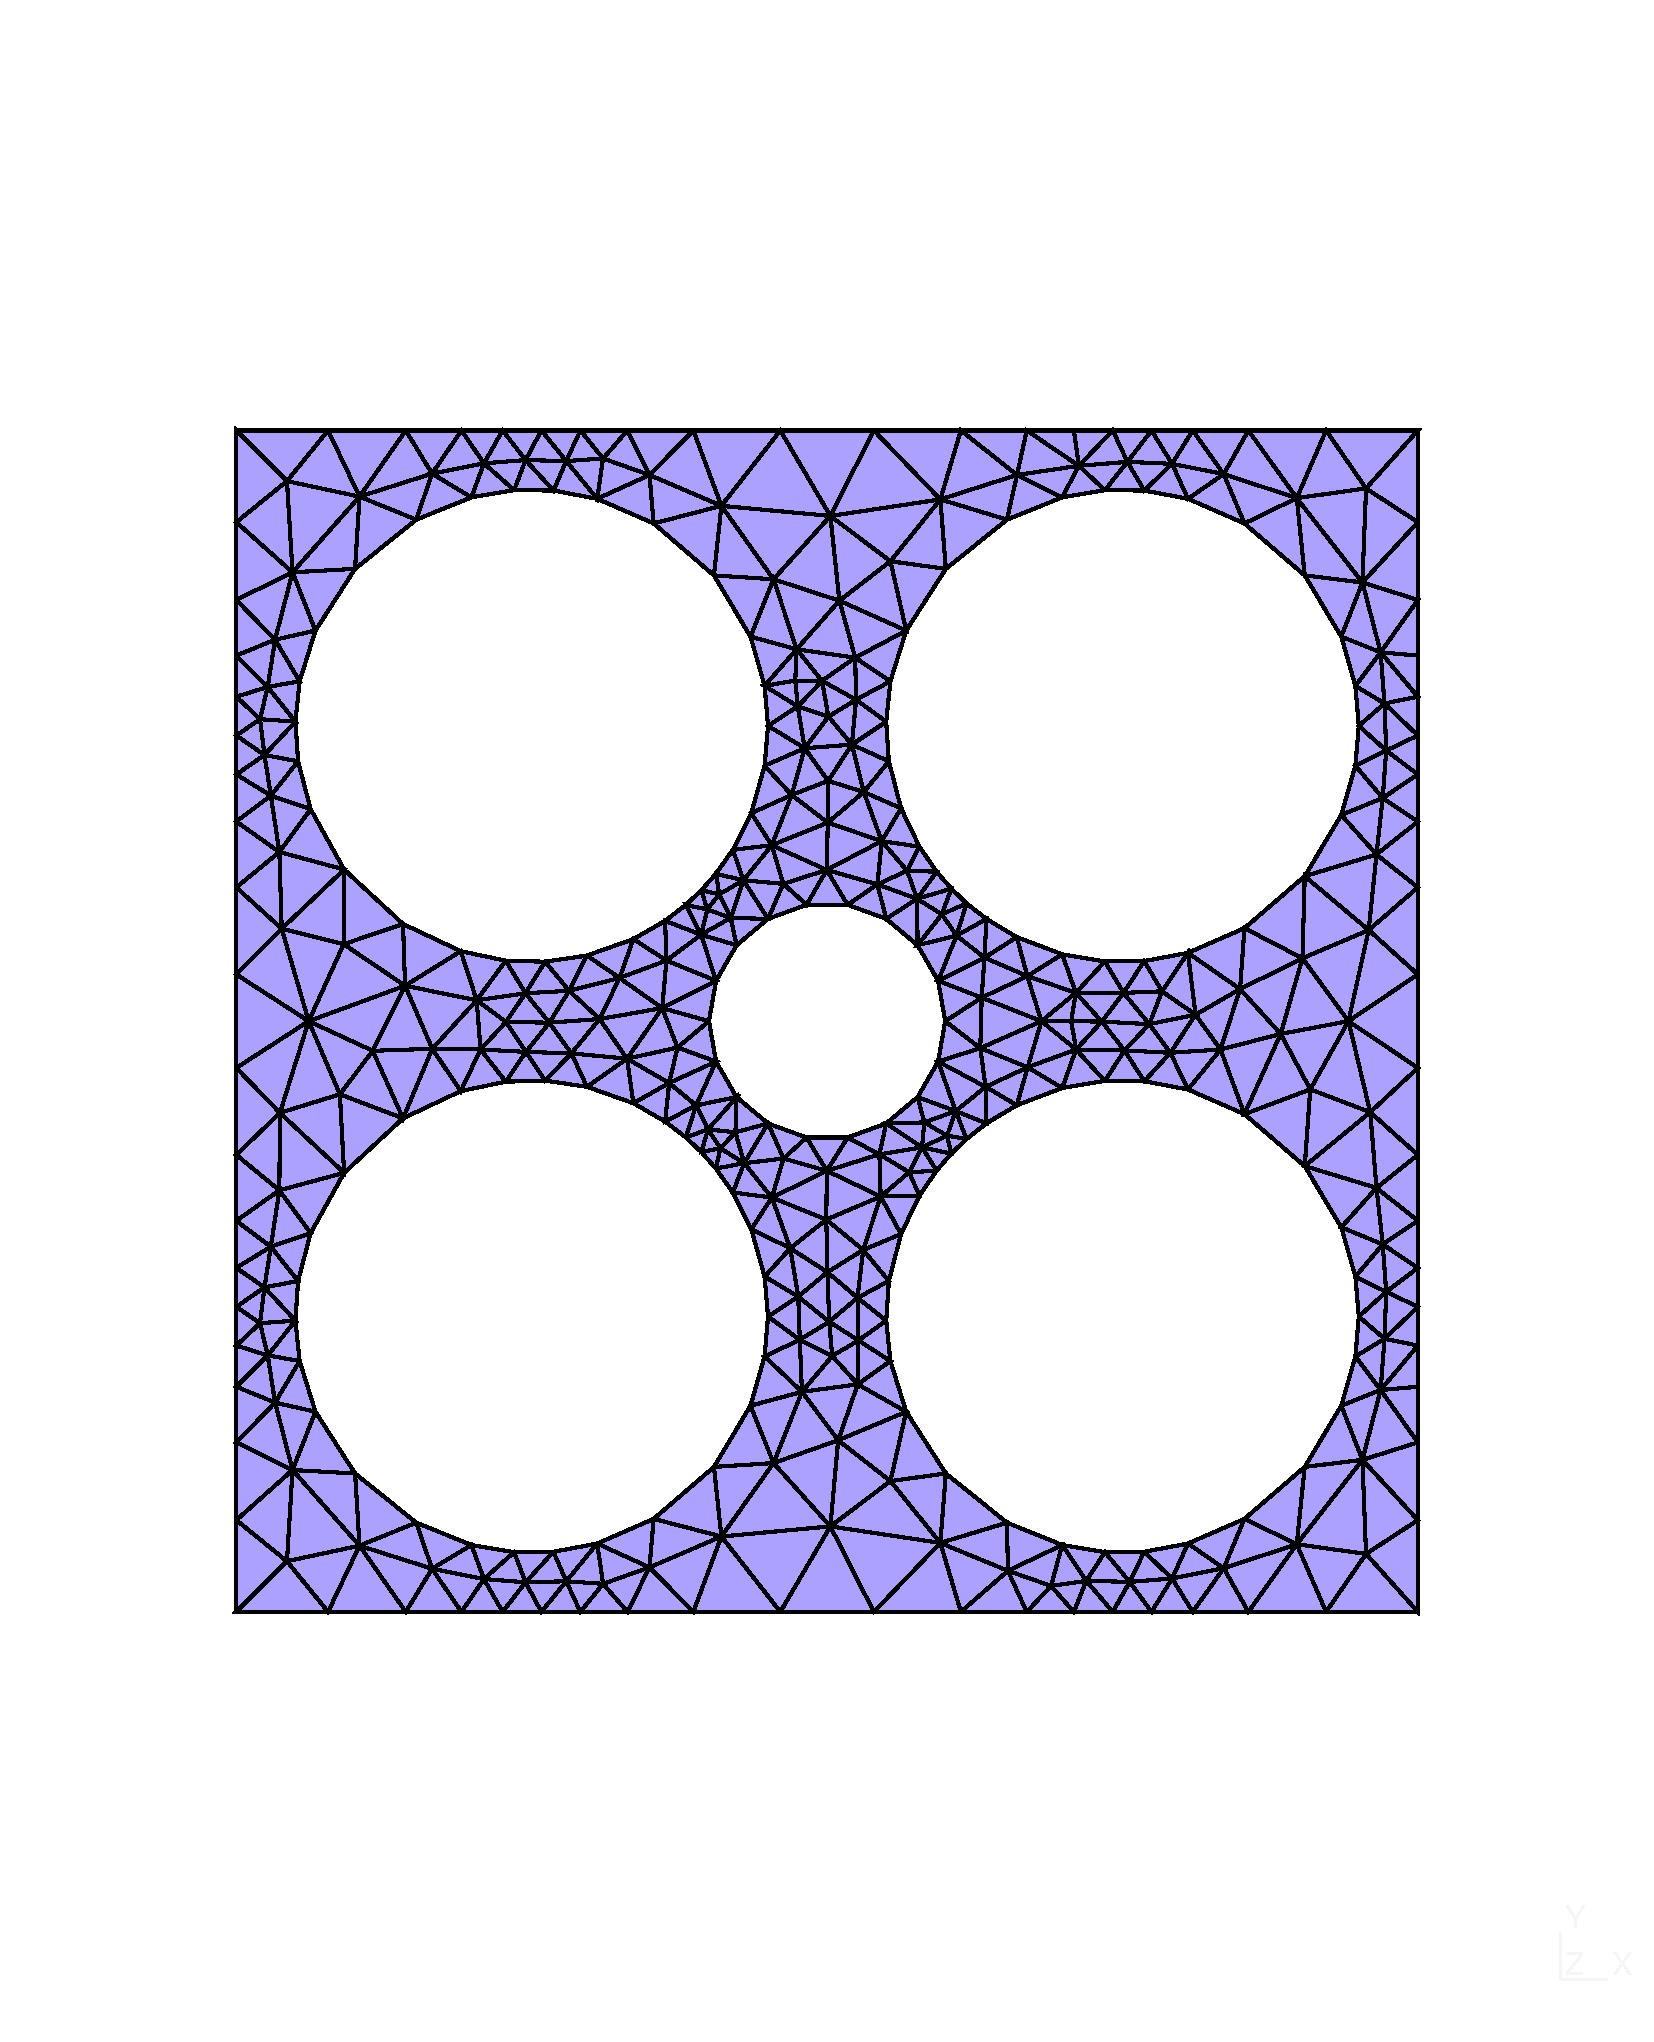
\includegraphics[width=\textwidth]{Figures_\version/tasks/5_star.pdf}
    \caption{Task 4}
    \label{fig:task4}
  \end{subfigure}
  \caption{Different domains introduced as different tasks.}
  \label{fig:tasks}
\end{figure}

